\section{Solutions \label{app:solutions}}
The solutions to the numerically modified problems in our collection can be found on \benchmarkrepo{}, where they are given as part of the Harbor task bundle. 

If a detailed solution is required, it is simplest to obtain this using an LLM that can solve the problem. Such an LLM can be identified using Table \ref{tab:detailed-results}. In our experience, Astra often gets not just the final answer but also the intermediate physics correct.

We now describe the solution to the inverse problem (\problemref{problem:autonomous-ode}), which no model solved.  The following fractional delay equation closely reproduces the displayed curve
on $0\le t\le 5$:
\[
f'(t)={}_0D_t^{1/5}f(t)-5\,{}_0D_t^{1/3}f(t)
       +500f(t-1)+550, \qquad t>0,
\]
with the initial data
\[
f(t)=-\frac{11}{10}\quad(-1\le t<0),
\qquad f(0)=1.0073\times10^{-5}.
\]
Here the fractional derivatives are Riemann--Liouville derivatives,
\[
{}_0D_t^\alpha f(t)=
\frac{1}{\Gamma(1-\alpha)}\frac{d}{dt}
\int_0^t(t-s)^{-\alpha}f(s)\,ds,
\qquad 0<\alpha<1.
\]

The solution of this equation is plotted in Figure \ref{desol} with dots overlaying the original curve. 
\begin{figure}[!h]
\begin{center}
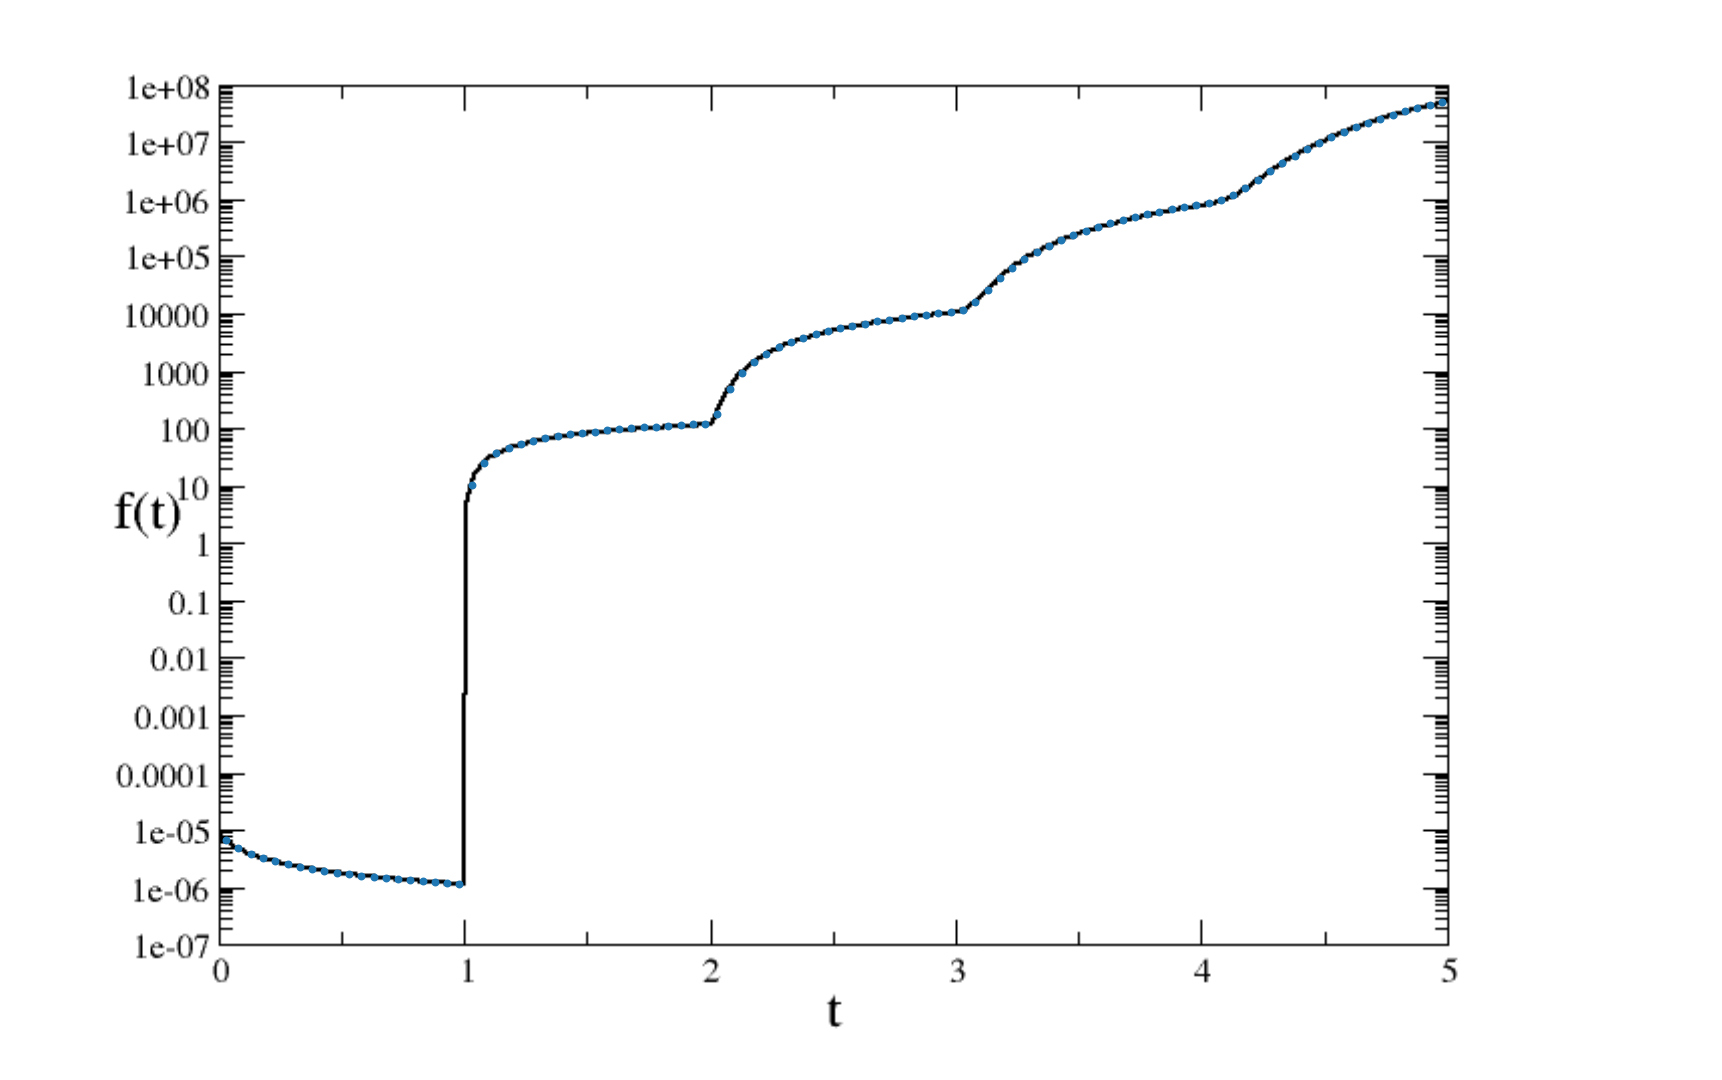
\includegraphics[width=\linewidth]{fig1_dots.png}
\end{center}
\caption{Numerical solution of the differential equation.\label{desol}}
\end{figure}

This solution plays upon the phrase ``differential equation'' since this equation involves both fractional and delay terms. From a strict perspective, this problem  might appear ``unfair.'' But, in real life, physicists are often faced with noisy data that they must use to infer the underlying physical process, and sometimes even relax the starting assumptions.  So, this question is representative of real research.

The solution above is not claimed to be unique and the reader may check that other equations with similar coefficients can also fit the curve. For this reason, this problem is resistant to a conversion along the lines of Box ~\ref{boxnumerical}.  The prompt asked the agents to output $0$ if no equation existed, and output the equation if they found one. We would have graded the agents positively for any equation that provided a good visual fit to the curve, but no agent was able to find such an equation.

It is worth noting that, in a private chat session, separate from the final API runs, Astra did guess that the equation would require fractional derivatives and delay terms. However, even there, it failed to perform an exhaustive search to determine the correct parameters.
%%% Local Variables:
%%% mode: LaTeX
%%% TeX-master: "paper"
%%% End:
